\documentclass[a4paper]{article}
\usepackage[utf8x]{inputenc}
\usepackage[portuguese]{babel}
\usepackage{graphicx}
\usepackage{a4wide}
\usepackage[pdftex,hidelinks]{hyperref}
\usepackage{float}
\usepackage{indentfirst}
\usepackage{subcaption}
\usepackage[cache=false]{minted}
\usepackage{amsmath}
\usepackage{listings}
\usepackage{color}

\definecolor{dkgreen}{rgb}{0,0.6,0}
\definecolor{gray}{rgb}{0.5,0.5,0.5}
\definecolor{mauve}{rgb}{0.58,0,0.82}

\lstset{frame=tb,
language=C++,
aboveskip=3mm,
belowskip=3mm,
showstringspaces=false,
columns=flexible,
basicstyle={\small\ttfamily},
numbers=none,
numberstyle=\tiny\color{gray},
keywordstyle=\color{blue},
commentstyle=\color{dkgreen},
stringstyle=\color{mauve},
breaklines=true,
breakatwhitespace=true,
tabsize=4
}

\newcommand{\x}{\times}

\begin{document}

\title{Computação Gráfica\\ Transformações Geométricas}
\author{Bárbara Cardoso (a80453) \and Márcio Sousa (a82400) \and Pedro Mendes (a79003)}
\date{\today}

\begin{titlepage}

    %título
    \thispagestyle{empty}
    \begin{center}
        \begin{minipage}{0.75\linewidth}
            \centering
            %engenharia logo
            
\includegraphics[width=0.4\textwidth]{eng.jpeg}\par\vspace{1cm}
            \vspace{1.5cm}
            %títulos
            \href{https://www.uminho.pt/PT}{\scshape\LARGE Universidade do Minho} \par
            \vspace{1cm}
            \href{https://www.di.uminho.pt/}{\scshape\Large Departamento de Informática} \par
            \vspace{1.5cm}

            \maketitle
        \end{minipage}
    \end{center}

\end{titlepage}

\tableofcontents

\pagebreak

\section{Introdução}
Este trabalho foi proposto no âmbito da unidade curricular de Computação Gráfica, e tem como objetivo desenvolver um motor gráfico genérico para representar objetos a 3 dimensões.

Nesta segunda fase do projeto estendemos as capacidades do motor gráfico anteriormente definido com a adição de transformações geométricas, para aplicar as antes definidas primitivas.

Para alem disto, também foi adicionada a definição de um torus ao gerador, especificamnente para suportar o anel de Saturno.

Com o intuito de demonstrar as capacidades do motor gráfico desenvolvido até ao presente, procedemos à criação de um modelo do Sistema Solar.

\section{Estrutura dos ficheiros usados pelo programa}\label{sec:estrutura-ficheiros}

Os ficheiros utilizados pelo programa estão definidos em formato \texttt{xml} com as seguintes tags:
\begin{itemize}
    \item \texttt{<scene>} Define o início de uma cena. Este funciona como se fosse um super grupo e não tem nenhum atributo.
    \item \texttt{<group>} Define um grupo de transformações, modelos e
        subgrupos, e aceita como atributos as cores com que os modelos devem ser pintados.
        Por exemplo,
        \texttt{<group R='1'> \ldots </group>} pinta todos os modelos de vermelho.
        Para além disto, os subgrupos deste irão herdar também estas cores a não ser
        que definam as suas próprias cores. Os atributos que podem ser usados 
        são R, G, B e A, que correspondem, respetivamente, a \textit{Red},
        \textit{Green}, \textit{Blue} e \textit{Alpha}. Alternativamente, pode também ser passado
        o parâmetro \textit{RAND} para que as cores sejam escolhidas aleatoriamente.
    \item \texttt{<models>} e \texttt{<model>} Definem os modelos a desenhar
        num grupo. O \texttt{<models>} contém uma lista do \texttt{<model>} e este tem o atributo
        \texttt{file} que indica qual o ficheiro \texttt{.3d} que vai ser usado.
    \item \texttt{<translate>}, \texttt{<rotate>} e \texttt{<scale>} Definem as
        transformações geométricas possíveis que podem ser usadas para transformar os
        modelos e os subgrupos. Os atributos de cada uma destas transformações são:
        \begin{itemize}
            \item \textbf{Translate:} X, Y, Z.
            \item \textbf{Rotate:} angle, X, Y, Z
            \item \textbf{Scale:} X, Y, Z
        \end{itemize}
\end{itemize}

\pagebreak
Exemplo de uma ficheiro de input:
\begin{minted}{xml}
<scene>
    <group R="1">
        <translate X="1" />
        <models>
            <model file="sphere.3d" /> <!-- Este modelo será vermelho -->
        </models>
        <group>
            <translate axisY="1" />
            <models>
                <model file="cone.3d" /> <!-- Este modelo será vermelho -->
            </models>
        </group>
        <group G="1">
            <models>
                <model file="torus.3d" /> <!-- Este modelo será verde -->
            </models>
        </group>
    </group>
    <group RAND="true">
        <translate X="5" axisY="0" axisZ="2" />
        <rotate angle="45" axisX="0" axisY="1" axisZ="0" />
        <models>
            <model file="box.3d" /> <!-- Este modelo tera cores aleatorias -->
        </models>
    </group>
</scene>
\end{minted}


\pagebreak

\section{Arquitetura do Projecto}

\subsection{Câmera}

A câmera não sofreu grandes alterações nesta segunda fase, em relação à fase anterior. Esta, apenas, foi movida para um \textit{namespace}, à parte.

\subsection{Model}

O model também não sofreu grandes alterações. Agora, para além de poder ser desenhado com cores aleatórias pode também ser desenhado sem cores (``herdando'' a última cor que tenha sido seleccionada).

\subsection{Render}

O render foi criado para mover a lógica de desenho para um \textit{namespace}, à
parte, e alterado para acomodar o resto das modificações.

\subsection{Group}

O \texttt{Group} é a nossa classe principal desta fase do projeto. Esta foi
desenhada para imitar o formato do xml, possuindo então uma sequência de
transformações, um conjunto de modelos e por fim os seus subgrupos, ficando
assim, com uma definição recursiva. Este é construído diretamente a partir do
xml, e disponibiliza uma função de desenho que pede a profundidade da árvore
de grupos e subgrupos que se pretende desenhar. Esta função funciona da
seguinte forma:

Caso o número passado como argumento seja maior do que 0, então esta começa por realizar todas
suas transformações, e de seguida desenha todos os modelos. Este passo tem a
atenção de aplicar as cores que possui, por passagem direta, ou por herança,
ou então desenha o modelo com cores aleatórias
(ver~\ref{sec:estrutura-ficheiros}). Por fim, chama recursivamente o método de
desenho sobre os subgrupos passando como argumento a profundidade recebida menos um.

Esta funcionalidade permite que sejam desenhadas apenas partes de árvore durante a execução usando as teclas
\texttt{[} e \texttt{]} para diminuir ou aumentar a profundidade da "árvore" de grupos que são desenhados, respetivamente. Por defeito, são desenhados todos os níveis.

\subsection{Transformations}

As transformações foram definidas como uma interface que obriga a
implementação do método \texttt{transform}. Foram definidas também 3 implementações
da mesma, \texttt{Rotate}, \texttt{Translate} e \texttt{Scale}, correspondentes
às 3 transformações possíveis.

\section{Novas Primitivas}

\subsection{Torus}

\begin{figure}[H]
    \centering 
    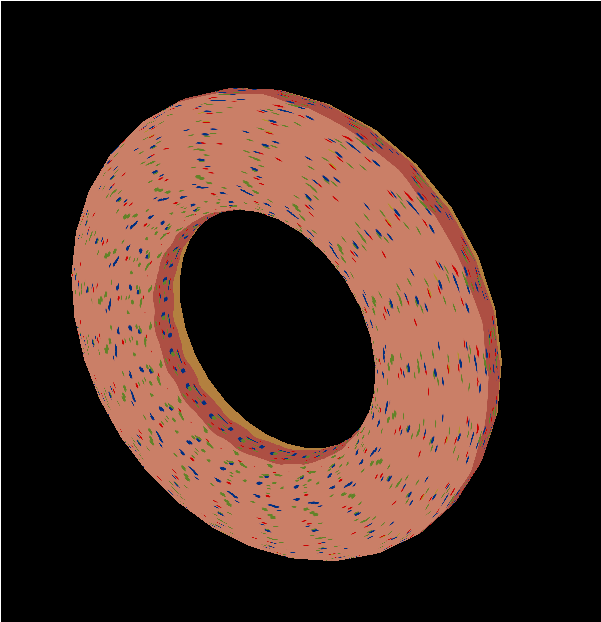
\includegraphics[width=0.5\textwidth]{torus.png}
    \caption{Torus: \textit{innerRadius}: 1, \textit{outerRadius}: 3, \textit{sides}: 10, \textit{rings}: 20}
\end{figure}

Um torus é definido por duas circunferências, uma interior e outra exterior, em
que a circunferência exterior tem um raio de $outerRadius$ e a circunferência interior um raio
de $outerRadius - 2 \x innerRadius$.
O $innerRadius$ é o raio de cada um dos anéis, que estão situado entre as duas circunferências. Os
centros destes anéis estão distanciados segundo um ângulo de $\alpha_{step}$,
usando coordenadas polares.

\begin{figure}[H]
    \centering
    \includegraphics{torus_diagram_full.png}
    \caption{Torus completo}
\end{figure}

Para cada par de anéis, são desenhados uma série de retângulos, que os interligam ambos, para fazer a ``parede'' do torus. Estes retângulos têm como vértices os pontos $p_0$, $p_1$, $p_2$ e $p_3$ que são calculados por coordenadas polares, e têm como centro de aplicação o centro do anel a que pertencem (ponto $B$). O espaçamento destes pontos segue, por sua vez, um ângulo de $\beta_{step}$.

\begin{figure}[H]
    \centering
    \includegraphics{torus_diagram_slice.png}
    \caption{Corte do torus com um par de anéis}
\end{figure}

\[B =  ((outerRadius - innerRadius) \x \sin \alpha, \quad (outerRadius - innerRadius) \x \cos \alpha, \quad 0)\]
\[B' = ((outerRadius - innerRadius) \x \sin (\alpha + \alpha_{step}), \quad (outerRadius - innerRadius)  \x \cos (\alpha + \alpha_{step}), \quad 0)\]

\[p_0 =
\begin{pmatrix}
    B_x + (innerRadius \x \cos \beta \x \sin \alpha)\\
    B_y + (innerRadius \x \cos \beta \x \cos \alpha)\\
    B_z + (innerRadius \x \sin \beta)\\
\end{pmatrix}
\]
\[p_1 =
\begin{pmatrix}
    B'_x + (innerRadius \x \cos \beta \x \sin(\alpha + \alpha_{step}))\\
    B'_y + (innerRadius \x \cos \beta \x \cos(\alpha + \alpha_{step}))\\
    B'_z + (innerRadius \x \sin \beta)\\
\end{pmatrix}
\]
\[p_2 =
\begin{pmatrix}
    B_x + (innerRadius \x \cos(\beta + \beta_{step}) \x \sin \alpha)\\
    B_y + (innerRadius \x \cos(\beta + \beta_{step}) \x \cos \alpha)\\
    B_z + (innerRadius \x \sin(\beta + \beta_{step})) \\
\end{pmatrix}
\]
\[p_3 =
\begin{pmatrix}
    B'_x + (innerRadius \x \cos(\beta + \beta_{step}) \x \sin(\alpha + \alpha_{step}))\\
    B'_y + (innerRadius \x \cos(\beta + \beta_{step}) \x \cos(\alpha + \alpha_{step}))\\
    B'_z + (innerRadius \x \sin(\beta + \beta_{step}))\\
\end{pmatrix}
\]

Para cada retângulo desenhado, o $\beta$ avança $\beta_{step}$ e para cada anel terminado $\alpha$ avança $\alpha_{step}$.

\section{Sistema Solar}

O sistema solar é constituído pelo Sol, que está no centro, 8 planetas e as respetivas luas.

Cada um destes astros é representado por uma esfera de raio 1 que depois é escalada para o tamanho pretendido. O sol é o astro que está situado no centro do sistema solar e por isto todas as transformações dependem deste.

Os planetas pertencem ao grupo do sol e que por sua vez têm o seu próprio subgrupo que contem as suas luas. Logo, os planetas herdam todas as caraterísticas do sol e as luas herdam as caraterísticas do seu respetivo planeta.
O planeta Saturno tem um anel que foi representado por um torus com a escala Z = 0.

Para colocar os planetas nas suas coordenadas foi escrito um curto \textit{script} em \textit{python} de forma a situar os planetas em torno do sol. Este usa raios predefinidos para cada planeta, que são as distâncias destes ao sol, e coordenadas polares para escolher uma posição aleatória.
Para as luas de cada planeta decidimos utilizar a mesma estratégia mas com a pequena diferença de que estas têm também uma componente vertical, ou seja, as suas posições podem ficar acima do equador.

\begin{figure}[H]
    \centering
    \includegraphics[width=\textwidth]{solar2.png}
    \caption{Um dos sistemas solares gerados}
\end{figure}

\section{Conclusões e Trabalho Futuro}
Esta fase do projeto possibilitou uma melhor compreensão do funcionamento das transformações geométricas do OpenGL e como estas podem ser usadas, sozinhas ou combinadas entre elas, de forma a criar cenários compostos por várias primitivas  gráficas previamente definidas.

Fazendo uma análise geral ao trabalho desenvolvido ao longo desta fase do projeto, podemos concluir que foram cumpridos todos os objetivos que nos foram propostos.

Como trabalho futuro, serão animados todos os astros do modelo do sistema solar representado, com o objetivo de obter a representação mais fidedigna possível.
\end{document}

